
% Copyright (c) 2015 - 2021 Mario Mlačak, mmlacak@gmail.com
% Licensed and published as Public Domain work.

% One chapter =========================================================
\chapter*{One}
\addcontentsline{toc}{chapter}{One}

\begin{flushright}
\parbox{0.8\textwidth}{
\emph{God is not external to anyone, but is present with all things, though
they are ignorant that he is so. \\
\hspace*{\fill}{\textperiodcentered \textperiodcentered \textperiodcentered \hspace*{0.2em} Plotinus} } }
\end{flushright}

\noindent
One is chess variant which is played on 26 x 26 board, with white and
darker violet fields, and with light purple and fuchsia pieces. Star
colors are reversed colors of ordinary pieces, i.e. fuchsia and light
purple. In algebraic notation, columns are enumerated from 'a' to 'z',
and rows are enumerated from '1' to '26'. A new piece is introduced,
Starchild.

\clearpage % ..........................................................
% Starchild ***********************************************************

\section*{Starchild}
\addcontentsline{toc}{section}{Starchild}

% \vspace*{-1.5\baselineskip}
\noindent
\begin{wrapfigure}[11]{l}{0.4\textwidth}
\centering
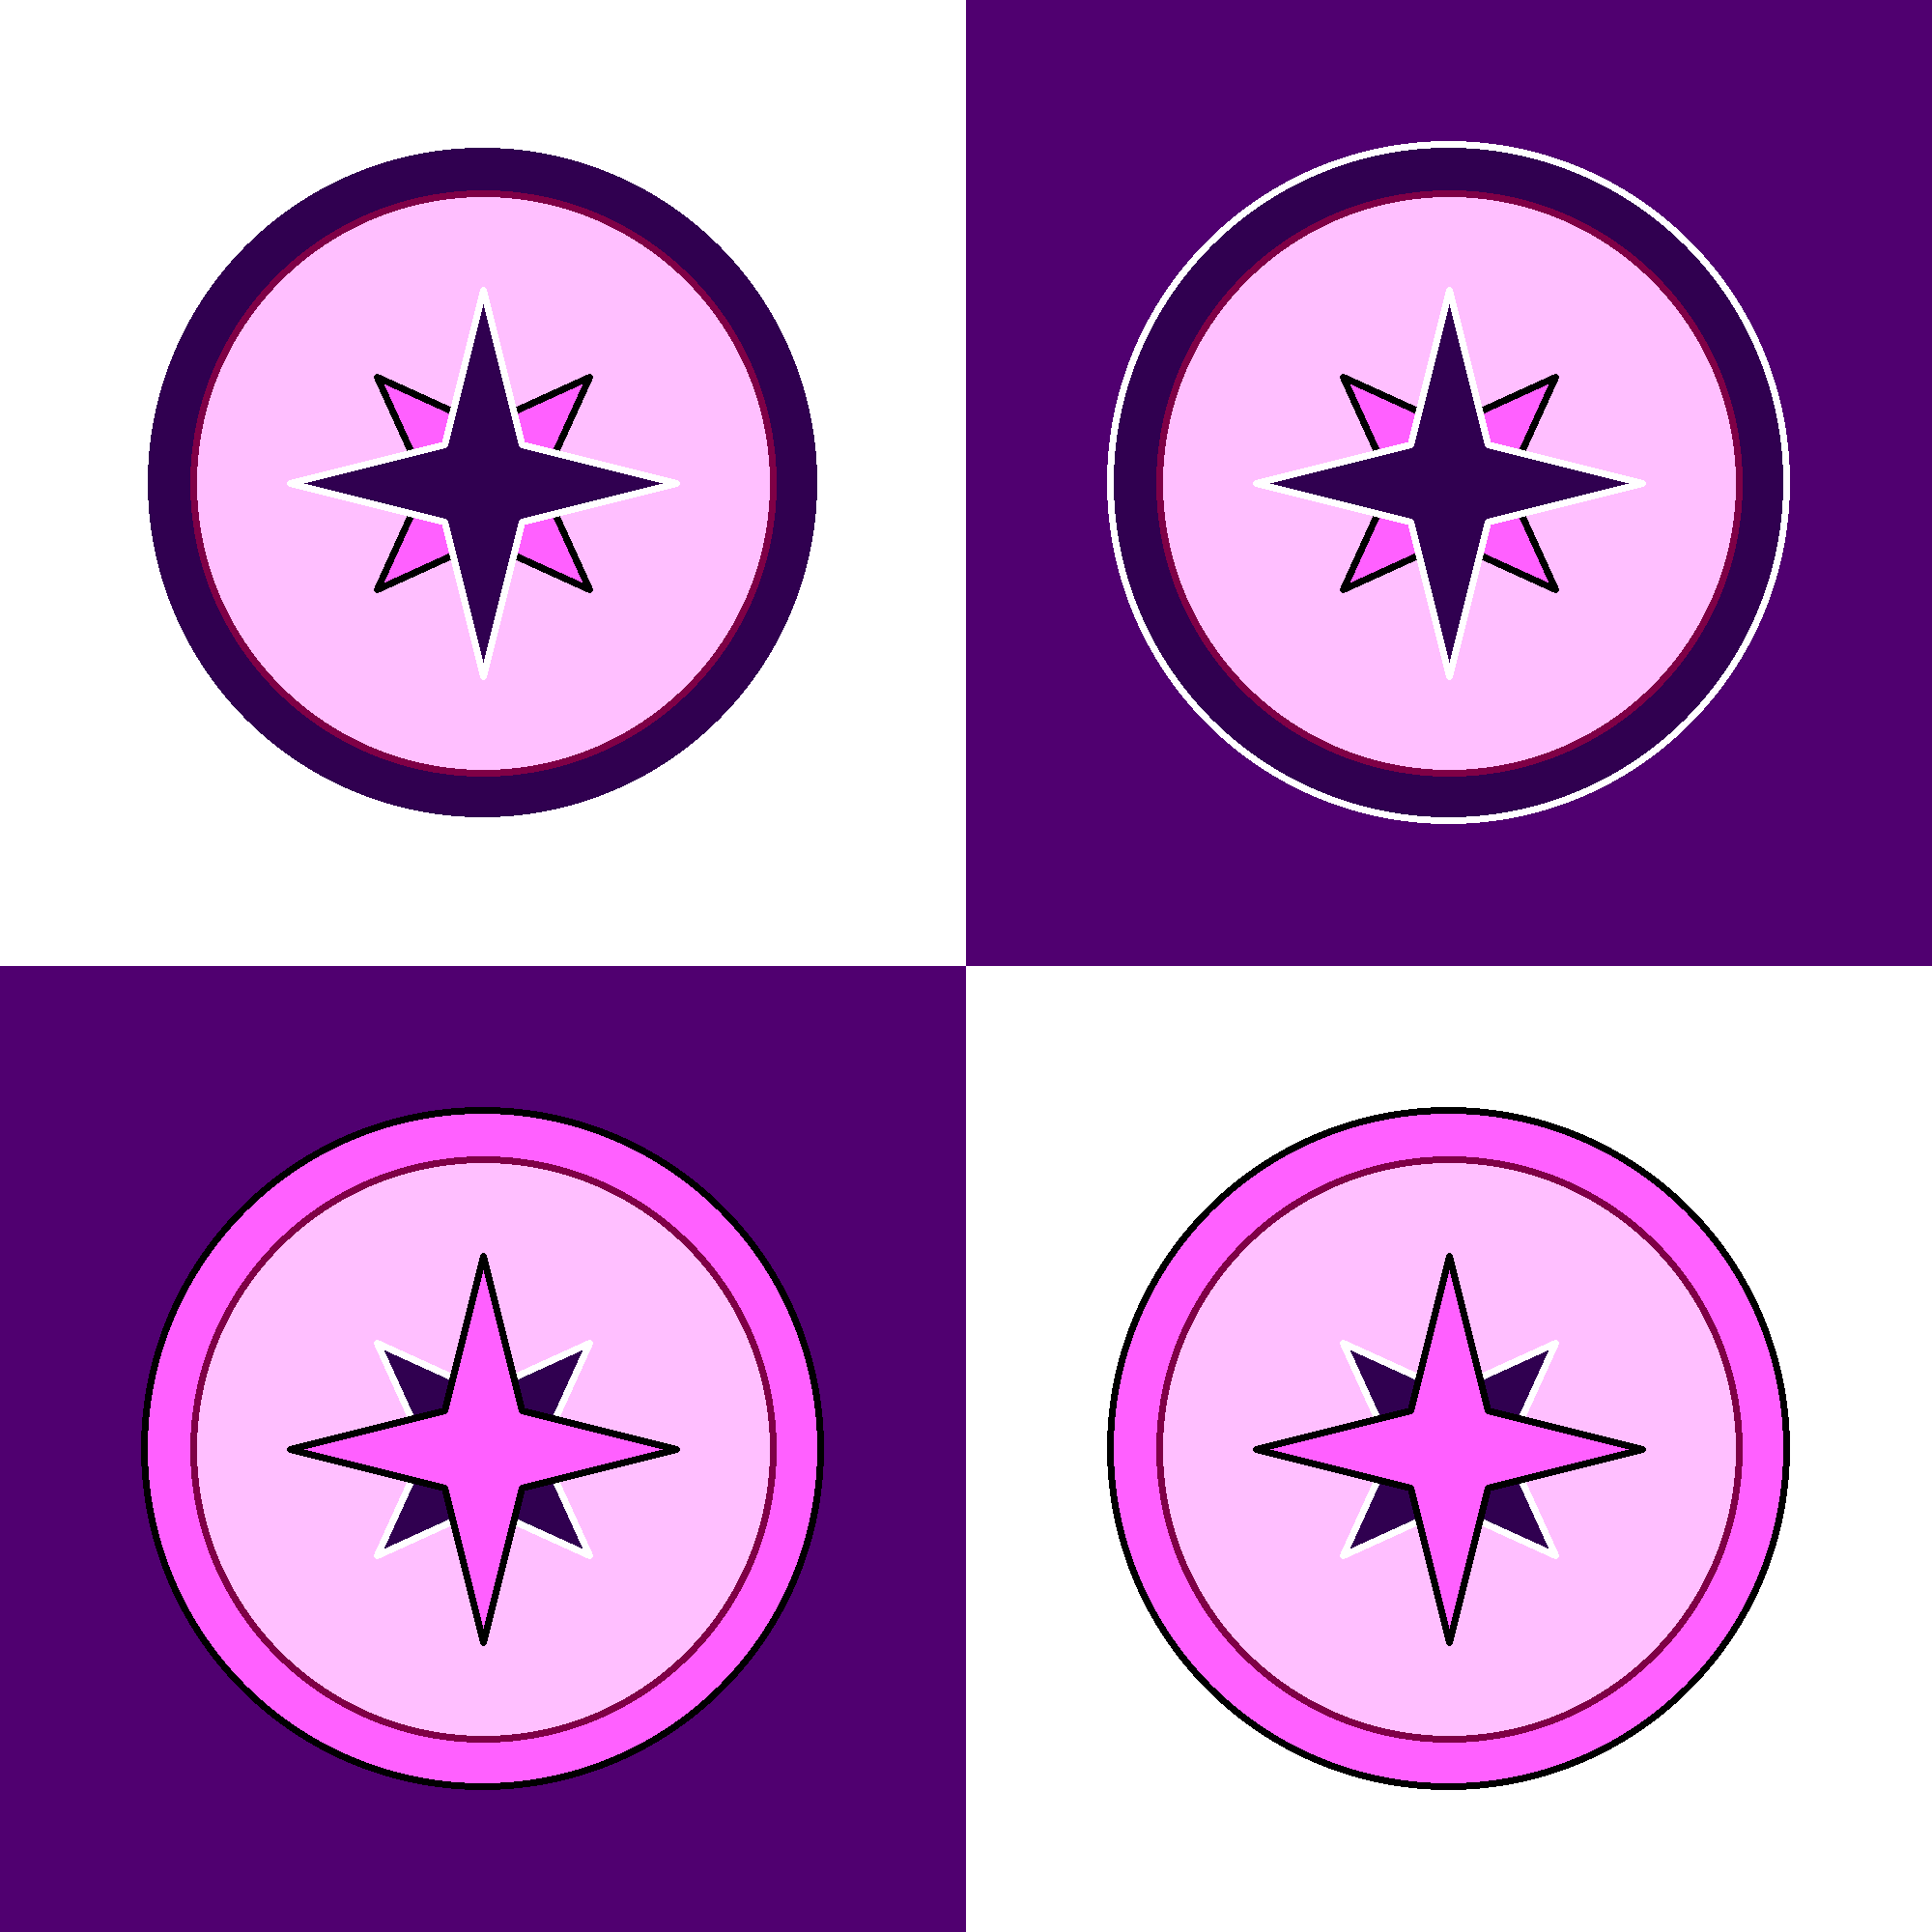
\includegraphics[width=0.4\textwidth, keepaspectratio=true]{pieces/16_starchild.png}
\caption{Starchild}
\label{fig:16_starchild}
\end{wrapfigure}
Starchild cannot capture any piece, cannot check or checkmate opponent's King.
Starchild is celestial piece, it can participate in demoting-to-Pawn syzygy.
Starchild can be demoted to Pawn.

Starchild cannot be converted, but can be activated. If activated, it does not spend
momentum while moving. Starchild can activate own Wave and Starchild on step-fields.
Starchild can activate any own piece (except King), opponent's Starchild and any Star
on its neighboring-fields.

% \vspace*{0.15\textheight}
\noindent
\begin{wrapfigure}[11]{l}{0.4\textwidth}
\centering
\includegraphics[width=0.4\textwidth, keepaspectratio=true]{pieces/star/22_one.png}
\caption{Star}
\label{fig:star/22_one}
\end{wrapfigure}
Starchild can't teleport. Starchild moves from starting to destination field in opposite
color in one step, without interacting with any piece on chessboard.

Starchild can resurrect any captured piece, except Kings, Stars, Monoliths. Waves and
Starchilds can be resurrected without resurrecting Starchild being oblationed. Starchild
can take any piece, except Kings, Waves, Stars and Monoliths, for a non-interactive,
viewing-only trance-journey.

In algebraic notation, symbol for Starchild is 'I'.

\clearpage % ..........................................................
% Movement ------------------------------------------------------------

\subsection*{Movement}
\addcontentsline{toc}{subsection}{Movement}

\vspace*{-1.1\baselineskip}
\noindent
\begin{figure}[!h]
% \begin{figure}[!t]
\includegraphics[width=1.0\textwidth, keepaspectratio=true]{examples/22_o/scn_o_01_starchild_movement.png}
\caption{Starchild movement}
\label{fig:scn_o_01_starchild_movement}
% \centering
\end{figure}

Starchild can move to any empty field in opposite color to the one it's located on.
Starchild is not hampered by any piece between starting and destination field.

Here, light Starchild in the middle moved from its starting position in one step.
It is now positioned at dark field, and so can access any empty light field in a
single step.

\clearpage % ..........................................................

\subsubsection*{Activating on step-fields}
\addcontentsline{toc}{subsubsection}{Activating on step-fields}

\vspace*{-1.1\baselineskip}
\noindent
\begin{figure}[!h]
% \begin{figure}[!t]
\includegraphics[width=1.0\textwidth, keepaspectratio=true]{examples/22_o/scn_o_02_starchild_activating_own_piece_init.png}
\caption{Activating Wave}
\label{fig:scn_o_02_starchild_activating_own_piece_init}
% \centering
\end{figure}

Starchild can activate own Waves and Starchilds on its step-fields, with 1 momentum. Here,
both light Waves and own Starchild can be activated. Neither light Rook nor any of other
opponent's pieces can be activated; some of them are also on the same color field as
activating Starchild.

\clearpage % ..........................................................

\vspace*{-2.1\baselineskip}
\noindent
\begin{figure}[!h]
% \begin{figure}[!t]
\includegraphics[width=1.0\textwidth, keepaspectratio=true]{examples/22_o/scn_o_03_starchild_activating_own_piece_end.png}
\caption{Wave activated}
\label{fig:scn_o_03_starchild_activating_own_piece_end}
% \centering
\end{figure}

Activated Wave moves the same as Starchild, i.e. to any field in opposite color to its starting
position. There it can activate any own piece (except King), and opponent's Wave, with 1 received
momentum. Here, light Wave A is now activated, and it can activate dark Wave or light Rook. It
cannot activate other opponent's pieces (here, dark Knight, Pegasus). Light Starchild and Wave B
can't be activated because they're on the same dark field as activating Wave.

\clearpage % ..........................................................

\subsubsection*{Activating Starchild}
\addcontentsline{toc}{subsubsection}{Activating Starchild}

\vspace*{-1.3\baselineskip}
\noindent
\begin{figure}[!h]
% \begin{figure}[!t]
\includegraphics[width=1.0\textwidth, keepaspectratio=true]{examples/22_o/scn_o_04_activating_starchild.png}
\caption{Activating Starchild}
\label{fig:scn_o_04_activating_starchild}
% \centering
\end{figure}

\hyperref[fig:10_wave]{Like Wave}, activated Starchild does not spend received momentum for moving;
if Starchild activates a piece, it transfers all of received momentum to it. In example similar to
previous, light Starchild is receiving 5 momentum after being activated by light Queen, received
momentum is then transfered from light Wave to dark Wave to dark Knight in its entirety.

\clearpage % ..........................................................

\subsubsection*{Neighboring-fields}
\addcontentsline{toc}{subsubsection}{Neighboring-fields}

% \vspace*{-0.9\baselineskip}
\noindent
\begin{wrapfigure}[5]{l}{0.4\textwidth}
\centering
\includegraphics[width=0.192307692\textwidth, keepaspectratio=true]{examples/22_o/scn_o_05_neighboring_fields.png}
\caption{Neighboring-fields}
\label{fig:scn_o_05_neighboring_fields}
\end{wrapfigure}
Neighboring-fields are all fields immediately surrounding a piece horizontally, vertically
and diagonally. They are the same as step-fields of a King.

\clearpage % ..........................................................

% \vspace*{1.1\baselineskip}
\subsubsection*{Activating on neighboring-fields}
\addcontentsline{toc}{subsubsection}{Activating on neighboring-fields}

% \vspace*{-0.9\baselineskip}
\noindent
\begin{wrapfigure}[7]{l}{0.4\textwidth}
\centering
\includegraphics[width=0.192307692\textwidth, keepaspectratio=true]{examples/22_o/scn_o_06_starchild_activating_on_neighboring_fields.png}
\caption{Activating piece}
\label{fig:scn_o_06_starchild_activating_on_neighboring_fields}
\end{wrapfigure}
Fields at which Starchild can activate a piece are neighboring-fields; pieces that can be
activated are own pieces (except King), and opponent's Starchild.

Note, Starchild cannot move to empty neighboring-fields, it can only activate a piece on its
neighboring-field.

Here, Starchild’s activation fields are enumerated. Opponent's Bishop and own King can't
be activated, so only own Pegasus can be, with 1 momentum.

\vspace*{-1.1\baselineskip}
\subsubsection*{Activating Wave}
\addcontentsline{toc}{subsubsection}{Activating Wave}

% \vspace*{-0.9\baselineskip}
\noindent
\begin{wrapfigure}[8]{l}{0.4\textwidth}
\centering
\includegraphics[width=0.192307692\textwidth, keepaspectratio=true]{examples/22_o/scn_o_07_starchild_activating_wave_on_neighboring_fields.png}
\caption{Activating Wave}
\label{fig:scn_o_07_starchild_activating_wave_on_neighboring_fields}
\end{wrapfigure}
Wave activated by Starchild on its neighboring-fields can activate a piece, with 1 momentum;
any own piece (except King), and opponent's Waves can be activated.

Wave can also move to any empty neighboring-field, regardless of color.

\hyperref[fig:scn_o_13_starchild_activated_wave_not_teleporting_init]{Activated Wave cannot teleport}.
Instead of teleporting, Wave would reappear on any empty portal-field around Star (or Monolith).
If there are no empty portal-fields, Wave would be oblationed.

\clearpage % ..........................................................

% \vspace*{2.1\baselineskip}
\subsubsection*{Moving a Star}
\addcontentsline{toc}{subsubsection}{Moving a Star}

% \vspace*{-0.9\baselineskip}
\noindent
\begin{wrapfigure}[5]{l}{0.4\textwidth}
\centering
\includegraphics[width=0.192307692\textwidth, keepaspectratio=true]{examples/22_o/scn_o_08_starchild_moving_star_init.png}
\caption{Moving into a Star}
\label{fig:scn_o_08_starchild_moving_star_init}
\end{wrapfigure}
Starchild can activate a Star the same way as any other piece, i.e. by capturing neighboring-field
at which Star is located. Activated Star receives 1 momentum.

\vspace*{2.1\baselineskip}
\noindent
\begin{wrapfigure}[4]{l}{0.4\textwidth}
\centering
\includegraphics[width=0.192307692\textwidth, keepaspectratio=true]{examples/22_o/scn_o_09_starchild_moving_star_end.png}
\caption{Star moving}
\label{fig:scn_o_09_starchild_moving_star_end}
\end{wrapfigure}
Once activated, Star can move to any empty neighboring-field, which all are enumerated in
example on the left.

\vspace*{2.3\baselineskip}
\noindent
\begin{wrapfigure}[9]{l}{0.4\textwidth}
\centering
\includegraphics[width=0.192307692\textwidth, keepaspectratio=true]{examples/22_o/scn_o_10_starchild_moving_star_activating.png}
\caption{Activating Starchild}
\label{fig:scn_o_10_starchild_moving_star_activating}
\end{wrapfigure}
Note, even if activated Starchild received more than 1 momentum, Star can move for only one step.

Here, Star received all of initial 3 momentum gathered by the Rook, since neither Wave nor Starchild expend momentum for its movement.
Nevertheless, activated Star can move for only one field.

\clearpage % ..........................................................

% \vspace*{1.1\baselineskip}
\subsubsection*{Not teleporting}
\addcontentsline{toc}{subsubsection}{Not teleporting}

% \vspace*{-0.9\baselineskip}
\noindent
\begin{wrapfigure}[4]{l}{0.4\textwidth}
\centering
\includegraphics[width=0.346153846\textwidth, keepaspectratio=true]{examples/22_o/scn_o_11_starchild_not_moving_monolith_init.png}
\caption{Moving into a Monolith}
\label{fig:scn_o_11_starchild_not_moving_monolith_init}
\end{wrapfigure}
Starchild can try to capture either step- or neighboring-field at which Monolith is located,
as if trying to teleport.

\vspace*{7.1\baselineskip}
\noindent
\begin{wrapfigure}[5]{l}{0.4\textwidth}
\centering
\includegraphics[width=0.346153846\textwidth, keepaspectratio=true]{examples/22_o/scn_o_12_starchild_not_moving_monolith_end.png}
\caption{Moving out of a Monolith}
\label{fig:scn_o_12_starchild_not_moving_monolith_end}
\end{wrapfigure}
Instead of teleporting, Starchild then emerges on any empty portal-field around Monolith
it tried to move. If there are no empty portal-fields, Starchild is oblationed.

\clearpage % ..........................................................

% \vspace*{1.1\baselineskip}
\subsubsection*{Not teleporting Wave}
\addcontentsline{toc}{subsubsection}{Not teleporting Wave}

% \vspace*{-0.9\baselineskip}
\noindent
\begin{wrapfigure}[4]{l}{0.4\textwidth}
\centering
\includegraphics[width=0.346153846\textwidth, keepaspectratio=true]{examples/22_o/scn_o_13_starchild_activated_wave_not_teleporting_init.png}
\caption{Moving into a Star}
\label{fig:scn_o_13_starchild_activated_wave_not_teleporting_init}
\end{wrapfigure}
Wave activated by Starchild cannot teleport, regardless if Wave was activated on Starchild's
step- or neighboring-field.

\vspace*{7.1\baselineskip}
\noindent
\begin{wrapfigure}[7]{l}{0.4\textwidth}
\centering
\includegraphics[width=0.346153846\textwidth, keepaspectratio=true]{examples/22_o/scn_o_14_starchild_activated_wave_not_teleporting_end.png}
\caption{Moving out of a Star}
\label{fig:scn_o_14_starchild_activated_wave_not_teleporting_end}
\end{wrapfigure}
Instead of teleporting, Wave emerges on an empty portal-field around Monolith or a Star through
which it tried to teleport.

If there is no empty portal-field around Monolith (or a Star), Wave is oblationed.

\clearpage % ..........................................................

% \vspace*{1.1\baselineskip}
\subsubsection*{Teleporting Wave}
\addcontentsline{toc}{subsubsection}{Teleporting Wave}

\vspace*{-0.9\baselineskip}
\noindent
\begin{figure}[!h]
% \begin{figure}[!t]
\includegraphics[width=1.0\textwidth, keepaspectratio=true]{examples/22_o/scn_o_15_star_moved_wave_teleportation.png}
\caption{Optional Wave teleportation}
\label{fig:scn_o_15_star_moved_wave_teleportation}
% \centering
\end{figure}

\vspace*{-0.3\baselineskip}
Wave activated by pieces other than Starchild can still teleport as usual. Stars in this variant
can be moved out of their default positions. Teleportation for Wave reaching a Star is optional,
step-fields behind a Star are still accessible. Here, light Wave could also activate light Queen. So,
\hyperref[fig:scn_d_09_teleport_wave_via_monolith]{Monolith is the only piece Wave cannot "pass-through"},
i.e. ignore as all the other pieces on chessboard.

\clearpage % ..........................................................

\vspace*{-2.1\baselineskip}
\noindent
\begin{figure}[!h]
% \begin{figure}[!t]
\includegraphics[width=1.0\textwidth, keepaspectratio=true]{examples/22_o/scn_o_16_star_moved_wave_off_board.png}
\caption{Wave teleported off-board}
\label{fig:scn_o_16_star_moved_wave_off_board}
% \centering
\end{figure}

Wave can end up with all step-fields off-board after teleportation, due to one or both Stars
moved out of their initial positions. In such a case, Wave is oblationed, the same as in
\hyperref[fig:scn_d_11_wave_teleported_off_board]{previous variant, Discovery}.

Wave is also removed from chessboard if, after teleportation, all of its step-fields are
blocked; this is again similar to
\hyperref[fig:scn_d_10_teleported_wave_blocked]{previous variant, Discovery}.

\clearpage % ..........................................................

% \vspace*{1.1\baselineskip}
\subsubsection*{Conversion immunity}
\addcontentsline{toc}{subsubsection}{Conversion immunity}

\vspace*{-0.9\baselineskip}
\noindent
\begin{figure}[!h]
% \begin{figure}[!t]
\includegraphics[width=1.0\textwidth, keepaspectratio=true]{examples/22_o/scn_o_17_starchild_conversion_immunity_init.png}
\caption{Conversion immunity}
\label{fig:scn_o_17_starchild_conversion_immunity_init}
% \centering
\end{figure}

\hyperref[sec:Mayan Ascendancy/Pyramid/Conversion]{Conversion} is a move in which activated
Pyramid reaches opponent's piece, if it's not King, on own side of board. Pyramid is then
oblationed, and reached piece is replaced by the same piece in opposite color.
Starchild cannot be converted, instead, original Starchild remains on chessboard;
conversioning Pyramid is still oblationed.

% ------------------------------------------------------------ Movement
\clearpage % ..........................................................
% Trance-journey ------------------------------------------------------

\subsection*{Trance-journey}
\addcontentsline{toc}{subsection}{Trance-journey}

% \vspace*{-1.3\baselineskip}
\vspace*{-1.1\baselineskip}
% \vspace*{-0.9\baselineskip}
\noindent
\begin{wrapfigure}[11]{l}{0.4\textwidth}
\centering
\includegraphics[width=0.346153846\textwidth, keepaspectratio=true]{examples/22_o/scn_o_18_trance_journey_init_starchild.png}
\caption{Starchild initiating}
\label{fig:scn_o_18_trance_journey_init_starchild}
\end{wrapfigure}
Trance-journey is initiated by either Shaman or Starchild, by activating another Starchild.
Activated Starchild then activates a piece, entranced piece then leaves onto trance-journey.
Any piece, own or opponent's, can be entranced, except Kings, Waves, Stars and Monoliths.

Between initiating piece and entrancing Starchild only Waves are allowed, but no other pieces.
Initiating Shaman or Starchild can themselves be activated by some other piece(s), not necessarily
in the same color.

\vspace*{-0.3\baselineskip}
% \vspace*{-0.1\baselineskip}
\noindent
\begin{wrapfigure}[10]{l}{0.4\textwidth}
\centering
\includegraphics[width=0.346153846\textwidth, keepaspectratio=true]{examples/22_o/scn_o_19_trance_journey_init_shaman.png}
\caption{Shaman initiating}
\label{fig:scn_o_19_trance_journey_init_shaman}
\end{wrapfigure}
Entranced piece must have the same color as initiating Shaman or Starchild, color of
entrancing Starchild do not need to match.

Here, entranced piece is dark Bishop, both initiating pieces are also dark, i.e. dark Shaman
in this example, and dark Starchild in previous example. Entrancing piece in both examples
is light Starchild.

Entranced piece can end its trance-journey on any empty step-field. If all are occupied, then it emerges
on any empty entrancing Starchild's neighboring-field. If there's none, then it emerges on empty initiating
Shaman or Starchild's neighboring-fields. If all are occupied, entranced piece is oblationed.

\clearpage % ..........................................................

\vspace*{-2.1\baselineskip}
\noindent
\begin{figure}[!h]
% \begin{figure}[!t]
\includegraphics[width=1.0\textwidth, keepaspectratio=true]{examples/22_o/scn_o_20_trance_journey_started_by_shaman.png}
\caption{Trance-journey}
\label{fig:scn_o_20_trance_journey_started_by_shaman}
% \centering
\end{figure}

Trance-journey pattern depends on color of entrancing Starchild. Here, light Starchild features
\hyperref[fig:scn_cot_14_light_shaman_trance_journey]{light Shaman's pattern}. Should entrancing
Starchild be dark, it would also produce
\hyperref[fig:scn_cot_16_dark_shaman_trance_journey]{dark Shaman's pattern}.

Trance-journey is optional, entranced piece could just move, with received momentum.
Here, dark Bishop is receiving 1 momentum, so it could move for 1 step.

\clearpage % ..........................................................

% \vspace*{-1.1\baselineskip}
\subsubsection*{Push-pull entrancement}
\addcontentsline{toc}{subsubsection}{Push-pull entrancement}

\vspace*{-0.9\baselineskip}
\noindent
\begin{wrapfigure}[7]{l}{0.4\textwidth}
\centering
\includegraphics[width=0.346153846\textwidth, keepaspectratio=true]{examples/22_o/scn_o_21_push_pull_trance_journey_init.png}
\caption{Initiating trance-journey}
\label{fig:scn_o_21_push_pull_trance_journey_init}
\end{wrapfigure}
Starchild initiating trance-journey could also be activated later in the same cascade, and act as an
entrancing Shaman. This is similar to push-pull entrancement in the
\hyperref[fig:star/scn_cot_33_push_pull_entrancement_start]{previous variant, Conquest of Tlalocan}.

\vspace*{3.9\baselineskip}
% \vspace*{-0.9\baselineskip}
\noindent
\begin{wrapfigure}[10]{l}{0.4\textwidth}
\centering
\includegraphics[width=0.346153846\textwidth, keepaspectratio=true]{examples/22_o/scn_o_22_push_pull_trance_journey_entrancing.png}
\caption{Push-pull entrancing}
\label{fig:scn_o_22_push_pull_trance_journey_entrancing}
\end{wrapfigure}
In previous eample, dark Starchild activated Wave A, which then activated Wave B. Here, Wave B is
"in the air", about to activate dark Starchild, which will then entrance dark Knight.

\clearpage % ..........................................................

% \vspace*{-3.1\baselineskip}
\noindent
\begin{figure}[!h]
% \begin{figure}[!t]
\includegraphics[width=1.0\textwidth, keepaspectratio=true]{examples/22_o/scn_o_23_push_pull_trance_journey_entranced.png}
\caption{Dark-pattern trance-journey}
\label{fig:scn_o_23_push_pull_trance_journey_entranced}
% \centering
\end{figure}

Starchild can initiate trance-journey by
\hyperref[sec:Terms/Push-pull activation]{push-pull activation},
if its color is the same as color of entranced piece; here both Starchild and Knight are dark.

Push-pull activation would work even if initiating Starchild has been activated by some other pieces,
which don't have to be in the same color.

\clearpage % ..........................................................

% \vspace*{-1.1\baselineskip}
\subsubsection*{Failed trance-journey}
\addcontentsline{toc}{subsubsection}{Failed trance-journey}

\vspace*{-1.1\baselineskip}
\noindent
\begin{figure}[!h]
% \begin{figure}[!t]
\includegraphics[width=1.0\textwidth, keepaspectratio=true]{examples/22_o/scn_o_24_trance_journey_failed.png}
\caption{Failed trance-journey}
\label{fig:scn_o_24_trance_journey_failed}
% \centering
\end{figure}

If all step-fields in a trance-journey are blocked by Kings, Stars or Monoliths, entranced Shaman is
\hyperref[sec:Terms/Oblation]{oblationed}, i.e. removed from chessboard as if captured by opponent.

For a trance-journey to fail, since it's optional, all capture-fields needs to be either empty or
blocked by own pieces, and all step-fields of a normal movement also needs to be blocked.

\clearpage % ..........................................................

\noindent
\begin{figure}[!h]
% \begin{figure}[!t]
\includegraphics[width=1.0\textwidth, keepaspectratio=true]{examples/22_o/scn_o_25_trance_journey_failed_2.png}
\caption{Failed new trance-journey}
\label{fig:scn_o_25_trance_journey_failed_2}
% \centering
\end{figure}

In addition to all step-fields being blocked, for a Starchild-induced trance-journey to fail, all
neighboring-fields of initiating piece and entrancing Starchild needs to be blocked as well.

In contrast to \hyperref[fig:scn_o_24_trance_journey_failed]{Shaman's failed trance-journey},
Starchild-induced trance-journey is blocked by any piece on its step-fields; here, own and
opponent's Pawns.

% ------------------------------------------------------ Trance-journey
\clearpage % ..........................................................

\subsection*{Syzygy}
\addcontentsline{toc}{subsection}{Syzygy}

\vspace*{-1.3\baselineskip}
\noindent
\begin{figure}[!h]
% \begin{figure}[!t]
\includegraphics[width=1.0\textwidth, keepaspectratio=true]{examples/22_o/scn_o_26_syzygy_monolith.png}
\caption{Demoting-to-Pawn syzygy}
\label{fig:scn_o_26_syzygy_monolith}
% \centering
\end{figure}

Starchild is celestial piece, it can participate in
\hyperref[fig:scn_d_16_syzygy_2_stars_init]{demoting-to-Pawn syzygy} in place of Stars and Monoliths.
\hyperref[fig:scn_d_18_syzygy_2_monoliths_init]{Again}, shortest step connecting Stars, Monoliths,
Starchilds is called syzygy-step, fields which are connected by syzygy-steps are called syzygy-fields.
For horizontal and vertical syzygy, syzygy-steps are the same as steps of Rook; for diagonal it’s
Bishop steps. Starchilds are also eligible to demotion.

\clearpage % ..........................................................

\vspace*{-2.1\baselineskip}
\noindent
\begin{figure}[!h]
% \begin{figure}[!t]
\includegraphics[width=1.0\textwidth, keepaspectratio=true]{examples/22_o/scn_o_27_syzygy_star.png}
\caption{Star-initiated syzygy}
\label{fig:scn_o_27_syzygy_star}
% \centering
\end{figure}

Star-initiated syzygy brings no additional interactions, i.e. it neither can demote own figure to Pawn,
nor it can resurrect any captured piece.

\clearpage % ..........................................................

\vspace*{-2.1\baselineskip}
\noindent
\begin{figure}[!h]
% \begin{figure}[!t]
\includegraphics[width=1.0\textwidth, keepaspectratio=true]{examples/22_o/scn_o_28_syzygy_starchild_init.png}
\caption{Resurrection syzygy start}
\label{fig:scn_o_28_syzygy_starchild_init}
% \centering
\end{figure}

Starchild-initiated syzygy is resurrection. One captured piece can optionally be resurrected by
replacing initiating Starchild, Starchild itself is then oblationed. Only captured pieces can be
resurrected. Kings, Stars and Monoliths cannot be resurrected. \\
\hyperref[fig:scn_d_17_syzygy_2_stars_steps]{Similar to demoting-to-Pawn}, only one resurrection per syzygy is
allowed; to resurrect another piece Starchild in syzygy has to move out of alignment, and then back in.

\clearpage % ..........................................................

\vspace*{-2.1\baselineskip}
\noindent
\begin{figure}[!h]
% \begin{figure}[!t]
\includegraphics[width=1.0\textwidth, keepaspectratio=true]{examples/22_o/scn_o_29_syzygy_starchild_end.png}
\caption{Queen resurrected}
\label{fig:scn_o_29_syzygy_starchild_end}
% \centering
\end{figure}

Here, resurrected Queen replaced initiating Starchild. Note, in this variant
\hyperref[sec:One/Promotion]{promotion is monogamous}, so the only light Queen
had to be captured, before it could be resurrected.

\clearpage % ..........................................................

\vspace*{-2.1\baselineskip}
\noindent
\begin{figure}[!h]
% \begin{figure}[!t]
\includegraphics[width=1.0\textwidth, keepaspectratio=true]{examples/22_o/scn_o_30_syzygy_starchild_resurrection.png}
\caption{Starchild resurrected}
\label{fig:scn_o_30_syzygy_starchild_resurrection}
% \centering
\end{figure}

Captured Waves and Starchilds can be resurrected, without initiating Starchild being oblationed. Chosen
piece can emerge on any empty neighboring-field around Starchilds in syzygy. If neighboring-fields are
all occupied, piece emerges on any empty portal-field around Stars, Monoliths in syzygy. If portal-fields
are occupied, piece emerges on any empty syzygy-field. If all are occupied, resurrection is not performed.

\clearpage % ..........................................................

\subsubsection*{Cascading syzygy}
\addcontentsline{toc}{subsubsection}{Cascading syzygy}

\vspace*{-1.2\baselineskip}
\noindent
\begin{figure}[!h]
% \begin{figure}[!t]
\includegraphics[width=1.0\textwidth, keepaspectratio=true]{examples/22_o/scn_o_31_syzygy_starchild_cascading.png}
\caption{Starchild cascading}
\label{fig:scn_o_31_syzygy_starchild_cascading}
% \centering
\end{figure}

Starchild initiating syzygy can activate pieces on a destination syzygy-field, and start a cascade.
Here, Bishop can move for 1 step, after Wave transfers 1 momentum from syzygy-initiating Starchild.

\clearpage % ..........................................................

\vspace*{-2.1\baselineskip}
\noindent
\begin{figure}[!h]
% \begin{figure}[!t]
\includegraphics[width=1.0\textwidth, keepaspectratio=true]{examples/22_o/scn_o_32_syzygy_double_starchilds.png}
\caption{Double Starchild}
\label{fig:scn_o_32_syzygy_double_starchilds}
% \centering
\end{figure}

Starchild initiating syzygy can activate another Starchild(s), creating double (triple, ...) syzygies,
which all have the same syzygy-steps, connecting the same celestial pieces. In such a move, only one
Starchild can have additional interactions, i.e. only one resurrection can be performed.

\clearpage % ..........................................................

\vspace*{-2.1\baselineskip}
\noindent
\begin{figure}[!h]
% \begin{figure}[!t]
\includegraphics[width=1.0\textwidth, keepaspectratio=true]{examples/22_o/scn_o_33_two_syzygies_shared_celestial_piece.png}
\caption{Shared celestial piece}
\label{fig:scn_o_33_two_syzygies_shared_celestial_piece}
% \centering
\end{figure}

Starchild initiating syzygy can activate another Starchild(s), creating two (or more) syzygies, which
share a syzygy-field. If syzygies also share celestial piece on that shared syzygy-field, only one
Starchild can have additional interactions, i.e. only one resurrection can be performed. This is so
even if any, or all, syzygies could be created without shared celestial piece.

\clearpage % ..........................................................

\vspace*{-2.1\baselineskip}
\noindent
\begin{figure}[!h]
% \begin{figure}[!t]
\includegraphics[width=1.0\textwidth, keepaspectratio=true]{examples/22_o/scn_o_34_two_syzygies_shared_field.png}
\caption{Shared syzygy-field}
\label{fig:scn_o_34_two_syzygies_shared_field}
% \centering
\end{figure}

If two (or more) syzygies are created which share a syzygy-field, but do not share celestial piece, two
(or more) Starchilds can have additional interactions, i.e. two (or more) resurrections can be performed,
one for each Starchild in a separate syzygy. This is so even if any other, non-celestial piece occupies
shared syzygy-field.

\clearpage % ..........................................................

\vspace*{-2.1\baselineskip}
\noindent
\begin{figure}[!h]
% \begin{figure}[!t]
\includegraphics[width=1.0\textwidth, keepaspectratio=true]{examples/22_o/scn_o_35_two_syzygies_shared_nothing.png}
\caption{Independent syzygies}
\label{fig:scn_o_35_two_syzygies_shared_nothing}
% \centering
\end{figure}

If two (or more) syzygies are created which do not share syzygy-field, two (or more) resurrections can be
performed, one for each Starchild in a separate syzygy.

\clearpage % ..........................................................

\subsubsection*{Reentering syzygy}
\addcontentsline{toc}{subsubsection}{Reentering syzygy}

\vspace*{-1.2\baselineskip}
\noindent
\begin{figure}[!h]
% \begin{figure}[!t]
\includegraphics[width=1.0\textwidth, keepaspectratio=true]{examples/22_o/scn_o_36_reentering_syzygies.png}
\caption{Reentering syzygy}
\label{fig:scn_o_36_reentering_syzygies}
% \centering
\end{figure}

Similar to \hyperref[fig:scn_d_20_syzygy_reentering_same_move]{Monolith reentering syzygy}, to get option to
resurrect captured piece, Starchild has to move from a normal, non-syzygy field into syzygy. Starchild already
in syzygy can move into the same (or the other) alignment, but cannot resurrect any piece. To be able to resurrect,
Starchild has to move out of alignment in a first move, and then on a next move it can move into syzygy.

% *********************************************************** Starchild
\clearpage % ..........................................................

\section*{Promotion}
\addcontentsline{toc}{section}{Promotion}
\label{sec:One/Promotion}

Promotion is non enforced, delayed variety, i.e. it's the same as in
\hyperref[sec:Age of Aquarius/Promotion]{previous chess variant}, Age of Aquarius.

Additionaly, promotion in this variant is monogamous.
Only one Queen in the same color can be present on chessboard at any given time.

\clearpage % ..........................................................

\section*{Rush, en passant}
\addcontentsline{toc}{section}{Rush, en passant}

\vspace*{-1.2\baselineskip}
\noindent
\begin{figure}[!h]
% \begin{figure}[!t]

\includegraphics[width=1.0\textwidth, keepaspectratio=true]{en_passants/22_one_en_passant.png}
\caption{En passant}
\label{fig:22_one_en_passant}
% \centering
\end{figure}

Rush and en passant are identical to those in \hyperref[fig:14_hemera_s_dawn_en_passant]{Hemera's Dawn variant}.
Own Pawns can be rushed for up to 11 fields in this variant.

\clearpage % ..........................................................

\section*{Castling}
\addcontentsline{toc}{section}{Castling}

Castling is the same as in Classical Chess, only difference is that King can move between 2 and 10 fields across.
All other constraints from Classical Chess still applies.

\noindent
\begin{figure}[!h]
% \begin{figure}[!t]
\includegraphics[width=1.0\textwidth, keepaspectratio=true]{castlings/22_o/one_castling.png}
\caption{Castling}
\label{fig:one_castling}
% \centering
\end{figure}

In example above, all valid King's castling moves are numbered.

\noindent
\begin{figure}[!h]
% \begin{figure}[!t]
\includegraphics[width=1.0\textwidth, keepaspectratio=true]{castlings/22_o/one_castling_right_04.png}
\caption{Castling short right}
\label{fig:one_castling_right_04}
% \centering
\end{figure}

In this example King was castling short to the right. Initial King's position is marked with "K".
After castling is finished, right Rook ends up at field immediately left to the King.

\clearpage % ..........................................................

\section*{Initial setup}
\addcontentsline{toc}{section}{Initial setup}

Compared to initial setup of Discovery, Starchild is inserted between Unicorn and Shaman
symmetrically, on both sides of chessboard. This can be seen in the image below:

\noindent
% \begin{figure}[t]
\begin{figure}[h]
\includegraphics[width=1.0\textwidth, keepaspectratio=true]{boards/22_one.png}
\caption{One board}
\label{fig:22_one}
% \centering
\end{figure}

\clearpage % ..........................................................
% ========================================================= One chapter
